\section{Modelling emissions}

To model the carbon emissions from single vehicle trips, the fuel consumption is modelled from data obtained from an onboard smartphone.

The data received from smartphones comes from a variety of sensors. For this experiment we used the accelerometer and GPS sensors. From the GPS sensor information on speed, heading and location is obtained, and from the accelerometer the size and direction of acceleration is gathered.

\subsection{Method from National Emission model}

In the COPERT IV emission modelling program, emission from warm combustion engines is modelled from the speed of the vehicle. As an example the emission $CO_2$ is modelled by modelling the fuel consumption of the vehicle, since the $CO_2$ emission is directly linked to the amount of fuel burned in the engine. Equation \ref{emission} is an example of how COPERT IV models the fuel consumption of a petrol driven passenger car as a function of the speed of the vehicle \cite{Ntziachristos2012}. There is a similar equation covering the fuel consumption of diesel cars. The constants $a-e$ are found by testing and differs by car type, engine size, year of manufacturing, and regulation. The COPERT IV program uses mean values for all tested vehicles within a particular class of vehicles.

\begin{equation}
	FC_{warm} = \frac{a + c*v + e*v^2}{1 + b*v + d*v^2}
	\label{emission}
\end{equation}

Figure \ref{FC} shows an example of the fuel consumption of passenger cars from 1999 versus speed. The consumption is measured in $l/km$, and is seen to have a minimum at app. $80 km/h$ for petrol cars and app. $60 km/h$ for diesel driven cars. The fuel consumption is high for low speeds due to the fact that the engine is underused, and the fuel consumption is high at high speeds due to increased wind forces on the vehicle. The equation is only defined for the speed range $10 - 130 km/t$
 
\begin{figure}[h]
	\centering
  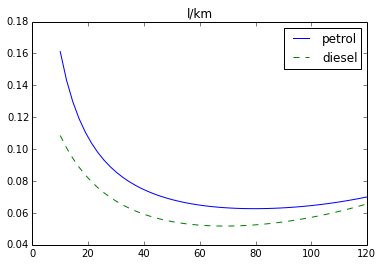
\includegraphics[width=0.45\textwidth]{fc_dieselpetrol}
  \caption{Fuel consumption versus speed for 1999 passenger car.}
  \label{FC}
\end{figure}

From fuel consumption the carbon dioxide emission can be modelled under the assumption of perfect combustion. If all carbon atoms in the fuel is oxidised into carbon dioxide, we only need to know how many carbon atoms there are in a liter of fuel.

\subsection{Single trip emission model}
The model developed in this paper builds upon the work from the national emission inventories. By using the instantaneous speed data obtained from Smartphones, and the fuel consumption versus speed curve from the COPERT program, instantaneous emissions can be calculated.

By assuming a constant speed between two measurements of the speed of the vehicle, and by measuring the distance between the two speed measurements, we calculate the fuel consumption for the distance by multiplying the distance with the fuel consumption given by equation \ref{emission}. The fuel consumption, and thus the carbon dioxide emission, for a single trip can then be calculated as the sum of the instantaneous consumptions.

One problem with the above method is that the fuel consumption model, defined in equation \ref{emission} is only valid for speeds between $10$ and $130 km/t$. This means that fuel consumption when the vehicle is idle (for instance waiting for green light at an intersection), is probably modelled too high.


\subsection{Emission model for accelerating vehicles}

To model the emission from accelerating vehicles, we first need to establish the different forms of driving modes. For each driving mode a emission model have to be employed.

In order to model the effect of vehicle acceleration, we divide the trip into six driving patterns, idle, forward acceleration, deceleration, cruise at constant speed, left turn and right turn. Reversing is not considered in this project, partly because we have no data and partly because it is an infrequent driving pattern. 

Gravity 

Position of smartphone

To detect acceleration


Turning

Cruise is characterised by
 For cruising the emission model from equation \ref{emission}, can be used, since the speed is constant.

Idle

The emission model for the braking and idle driving mode, can be the same, since regenerative braking is not used in many passenger cars with only a combustion engine.

K-means



 